\section{Υπολογισμός παραγώγων με τη συνεχή συζυγή μέθοδο} 

Όπως αναλύθηκε και στην προηγούμενη παράγραφο, δημιουργώντας την επαυξημένη αντικειμενική συνάρτηση μπορούμε επιλύωντας μονο τη συνεχή συζυγή εξίσωση (\ref{eq:FAE}), να λάβουμε την απλή έκφραση των παραγώγων μέσω της σχέσης \ref{eq:CAsens}. 

Όπως και η primal εξίσωσή μας (\ref{eq:primal}), και η συζυγής εξίσωση θα λυθεί αριθμητικά. Αν και ίσως διαθέτει αναλυτική λύση, τις τιμές της κύριας μεταβλητής $\delta$ ή $u$ τις έχουμε σε διακριτή μορφή στις θέσεις των κόμβων επομένως είναι ευκολότερο να την επιλύσουμε αριθμητικά ξανά με Runge Kutta 4ης τάξης ξεκινώντας απο τον τελευταίο κόμβο που ορίζουμε την συνοριακή συνθήκη. Έτσι, ξαναγράφουμε την εξίσωση \ref{eq:FAE} ως:

\begin{equation}
f(x,\Psi) = \dfrac{d\Psi}{dx} =  \dfrac{U\pi\mu}{2Au^3(x)} +  \dfrac{\Psi}{Avu(x)}\nu_0(x) 
    \label{eq:transFAE}
\end{equation}

Με $$A = \Big(\dfrac{2}{\pi} - \dfrac{1}{2}\Big)$$

\paragraph{Σημείωση:} Επειδή η επίλυση της \ref{eq:FAE} χρησιμοποιεί δεδομένα που προέκυψαν απο την πρώτη αριθμητική ολοκλήρωση, είναι επηρεπής σε συσσώρευση σφαλμάτων. Γι αυτό τον λόγο, για να βελτιώσουμε την ακρίβειά της χωρίς να αυξήσουμε πολύ τον αριθμό των κόμβων σε ολόκληρο το πρόβλημα, χρησιμοποιήσαμε διπλάσιο αριθμό κόμβων για την ολοκλήρωση της FAE και οι ενδιάμεσες τιμές λήφθηκαν με γραμμική παρεμβολή απο το πεδίο τους πάχους του οριακού στρώματος που προκύπτει απο την επίλυση της primal εξίσωσης. Η μεθοδολογία αναλύεται παρακάτω.  

\subsection{Επίλυση FAE με Runge Kutta 4ης τάξης}

$\Delta x' = -\Delta x / 2$

Κόμβοι συζυγούς πεδίου: $N_j = 2N_i - 1$


\begin{align*}
    k^1 &= \Delta x'f\Big(x^{j+1},\Psi^{j+1}\Big)\\[10pt]
    k^2 &= \Delta x'f\Big(x^{j+1} + \dfrac{\Delta x'}{2}, \Psi^{j+1} + \dfrac{k^1}{2}\Big)\\[10pt]
    k^3 &= \Delta x'f\Big(x^{j+1} + \dfrac{\Delta x'}{2}, \Psi^{j+1} + \dfrac{k^2}{2}\Big)\\[10pt]
    k_4 &= \Delta x'f\Big(x^j,\Psi^{j+i} + k_3\Big)
\end{align*}

$$y^{j} = y^{j+1} - \dfrac{1}{6}(k_1 + 2k_2 + 2k_3 + k_4) $$

\begin{figure}[h!]
    \centering
    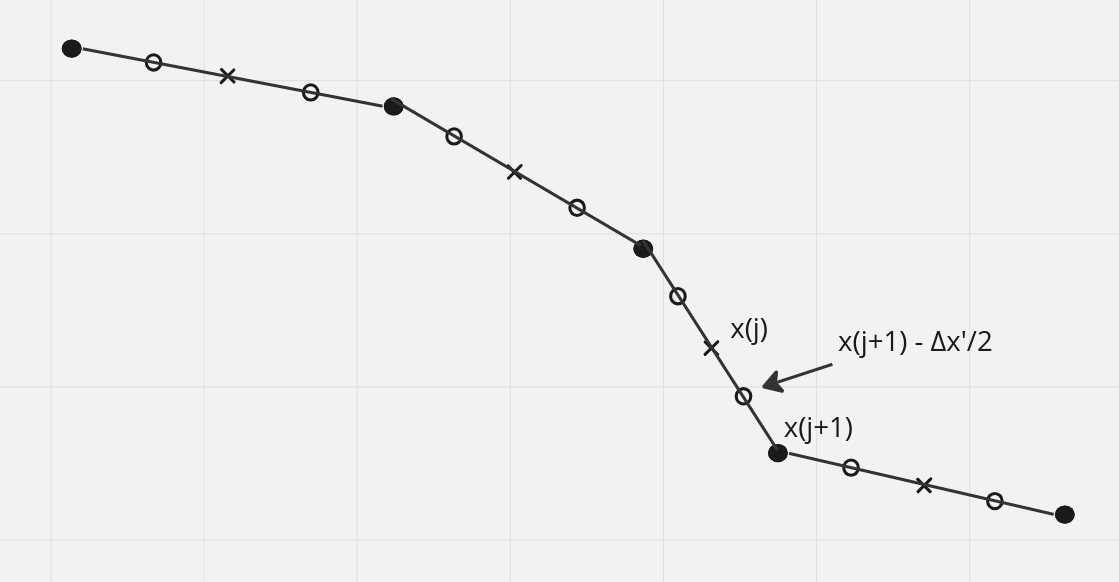
\includegraphics[width=0.8\textwidth]{figures/2nd_runge.png}
    \caption{Γραμμική παρεμβολή στις τιμές του $\delta$}
    \label{fig:interp}
\end{figure}

\subsection{Ολοκλήρωση - Υπολογισμός παραγώγων ευαισθησίας}

Οπότε πλέον μπορούμε να ολοκληρώσουμε την ποσότητα στο δεξί μέλος της σχέσης \ref{eq:CAsens} για να υπολογίσουμε τις παραγώγους ευαισθησίας της αντικειμενικής συνάρτησης. Αφού οι τιμές του ολοκληρώματος διατίθενται σε διακριτή μορφή, θα υπολογίσουμε το ολοκλήρωμα με τη μέθοδο των τραπεζίων:

\begin{align}
    \dfrac{\delta F}{\delta b_n} = - \sum^{N-1}_{i=0}\Bigg[\Big(\dfrac{\Psi_i}{v}u_i\dfrac{\delta \nu_0}{\delta b_n}\big|_i + \dfrac{\Psi_{i+1}}{v}u_{i+1}\dfrac{\delta \nu_0}{\delta b_n}\big|_{i+1}\Big)\dfrac{(x_{i+1} + x_i)}{2}\Bigg]
\end{align}

Το συζυγές πεδίο που προκύπτει απο τη συνεχή και τη διακριτή συζυγή μέθοδο παρατίθεται στο σχήμα \ref{fig:cadaComp}.

\begin{figure}[h!]
    \begin{center}
        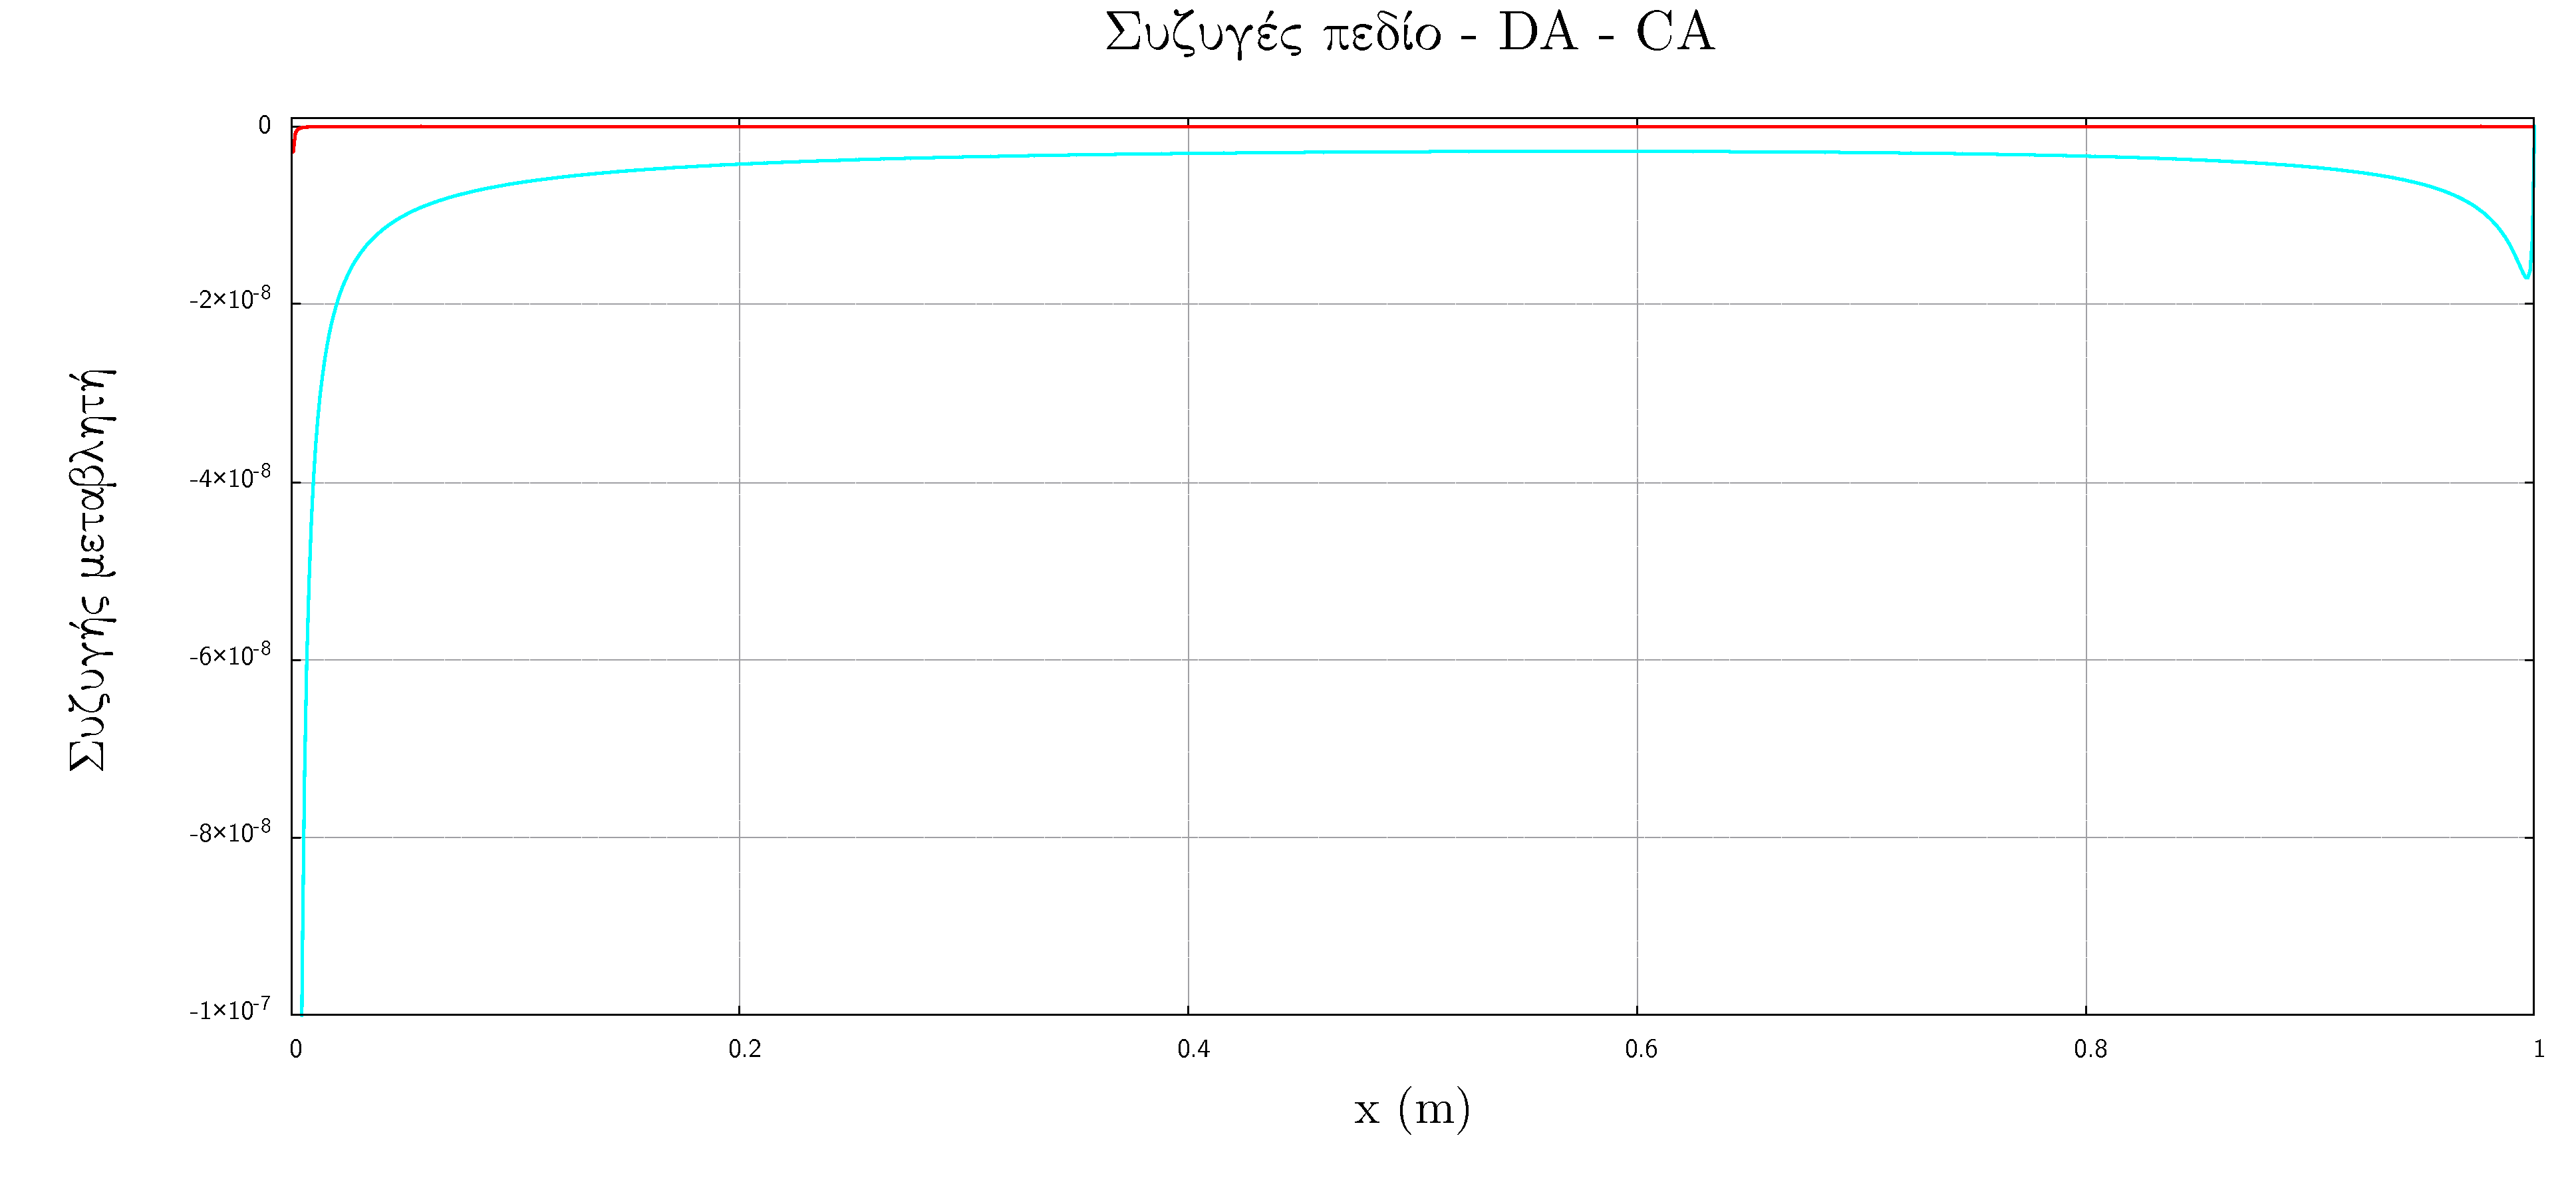
\includegraphics[width=0.95\textwidth]{figures/ca-vs-da.pdf}
    \end{center}
    \caption{Σύγκριση συζυγούς πεδίου συνεχής και διακριτής μεθόδου}
    \label{fig:cadaComp}
\end{figure}

\newpage

Παρατηρούμε μια έντονη διαφορά στην τάξη μεγέθους των αποτελεσμάτων των πεδίων ωστόσο συμφωνούν στη μορφή τους (συγκρίνωντας με το σχήμα \ref{fig:DAfield}). Αυτό είναι αναμενόμενο εν μέρει, διότι απο διαστατική ανάλυση της διακριτής συζυγής μεταβλητής και της συνεχής διακρίνουμε το εξής. Η διακριτή συζυγής μεταβλητή έχει μονάδες δύναμης (Ν), ενώ η συνεχής συζυγή μεταβλητή έχει $N/m^2$. Αυτό μπορεί να ερμηνευθεί ως εξής. Η διακριτή συζυγής μεταβλητή αφορά μια ποσότητα ανάλογη της δύναμης τριβής που συνεισφέρει ο κάθε κόμβος. Απο την άλλη, η συνεχής συζυγής μεταβλητή μπορεί να αφορά μια ποσότητα ανάλογη της διατμητικής τάσης. Έτσι, οι τιμές του διακριτού συζυγούς πεδίου εξαρτώνται απο το μέγεθος της διακριτοποίησης και τον αριθμό των κόμβων, ανώ η συνεχής, αφού αφορά την τιμή της αντικειμενικής συνάρτησης ανηγμένη σε μονάδα επιφάνειας, αναμένεται να είναι ανεξάρτητη του πλήθους των κόμβων. Δηλαδή, αναμένεται πως αν είχαμε μια διακριτοποίηση στην οποία η επιφάνεια κάθε κελιού ήταν ίση με 1 $m^2$, και παράλληλα το πλήθος των κόμβων είναι ικανοποιητικό ως προς την ακρίβεια, θα βλέπαμε πολύ κοντινότερες καμπύλες των συζυγών πεδίων.  




